\documentclass[a4paper]{scrartcl}

\usepackage[utf8]{inputenc}
\usepackage[english]{babel}
\usepackage{lmodern} 
\usepackage[T1]{fontenc}
\usepackage{booktabs}
\usepackage{multirow}
\usepackage{wrapfig}
\usepackage{caption}



% PAKETE
\usepackage{siunitx}
\usepackage{amsmath}
\usepackage{amssymb}
\usepackage{graphicx}
\usepackage{placeins}
\usepackage{longtable}
\usepackage{enumitem}
\usepackage{bbm}



% EINSTELLUNGEN
\sisetup{seperr,repeatunits=false}
\numberwithin{equation}{section}
\numberwithin{figure}{section}
\numberwithin{table}{section}

% EIGENE FUNKTIONEN
\newcommand{\re}{\operatorname{Re}}
\newcommand{\im}{\operatorname{Im}}
\newcommand{\gquote}[1]{\glqq #1 \grqq}

\newcommand{\eq}[2]{\begin{equation}#1\label{#2}\end{equation}}
\newcommand{\eqand}[0]{\hspace{.25cm} \bigwedge \hspace{.25cm}}
\newcommand{\grafik}[2]{\begin{figure}[h]\centering \includegraphics[width=10cm]{#1.eps}  \caption{#2} \label{#1} \end{figure} }
\newcommand{\grafikq}[3]{\begin{figure}[h]\centering \includegraphics[width=10cm]{#1.eps}  \caption[#2]{#3} \label{#1} \end{figure} }
\newcommand{\tbl}[3]{\begin{table}[h]\caption{#1}\label{#2}\begin{center}#3\end{center}\end{table}}
\newcommand{\Abbildung}[1]{\textsl{Abbildung \ref{#1}}}
\newcommand{\AbbildungI}[1]{\textsl{(Abbildung \ref{#1})}}
\newcommand{\Tabelle}[1]{\textsl{Tabelle \ref{#1}}}
\newcommand{\TabelleI}[1]{\textsl{(Tabelle \ref{#1})}}
\newcommand{\Formel}[1]{(\ref{#1})}
\renewcommand{\d}{\mathrm{d}}
\newcommand{\ve}[1]{\mathbf{ #1} }

\title{Ma 2: Low Energy Electron Diffraction (LEED) on Surfaces}
\subtitle{Tutor: Y. Kahn}
\author{Benjamin Huber, Carolin Wille}
\date{November 7, 2011}

\begin{document}
\thispagestyle{empty}
\maketitle
\tableofcontents
\clearpage


\section{Introduction}
\subsection{Matterwaves}
Following the principle of the wave-matter dualism, de Broglie proposed in 1924, that any particle of momentum $p$ or mass $m$ and energy $E$ can be also described as a wave of wavelength 
\eq{\lambda = \frac{h}{p} =\frac{h}{2mE} \;,}{lambda}
where $h=4.135667516(91)\times 10^{-15} \text{eVs}$ is the Planck constant. Therefore, electron scattering on surfaces can lead to intereference phenomena, if the electron wave length is of the order of the lattice constant. The de Broglie wave length of an electron, that is accelerated with a voltage $V_0$ is given by 
\eq{\lambda= \frac{\SI{12.26}{\AA}}{\sqrt{V_0}} \; }{lV}
and a typical eletron energy range from 50 to 500 eV corresponds to wavelengths between 0.5 and 2 $\AA$. Relativistic corrections have not to be taken into account in this energy range, as the ratio between velocity and speed of light for an electron accelerated with $V = \SI{500}{V}$ is given by
\eq{\frac{v}{c}=\sqrt{1-\frac{1}{(\frac{eV}{mc^2}+1)^2}} =0.04 \; .}{} 
and the relativistic correction given by the Lorentz factor $\gamma$ according to $\lambda_\text{rel.} = \frac{\lambda}{\gamma}$ is $\frac{1}{\gamma} = \sqrt{1-\frac{v^2}{c^2}}= 0.9992$. The acceleration for which relativistic effects would cause a deviation of $1\percent$ is given by
\eq{E=(\gamma -1)mc^2= \left(\frac{1}{0.99}-1\right)mc^2=\SI{5160}{eV}\;. }{}

\subsection{Constructive Interference for a surface scattering event}
Just as the Bragg Condition for constructive interference and the more advanced Laue theory, that can also determine the intensities of the scattered waves in solid state physics, these concepts can be applied for surface scattering as well. Analogue to the Bragg condition, the condition for constructive interference 
\eq{n \lambda = a_{h,k} (\sin \varphi - \sin \varphi_0 ) \; \qquad n \in \mathbb N }{bragg}
can be derived from a simple geometrical consideration shown in figure \ref{bragg}. The length $a$ is given by
\eq{a_{h,k} = |h \ve a_1 + k \ve a_2|\;, \qquad h,k \in \mathbb N \; , }{}
where $\ve a_1$ and $\ve a_2$ are the lattice vectors of the surface layer.

The scattering process can also be described by the usage of the reciprocal lattice vectors $\ve a_{1,2}^* \perp \ve a_{2,1}$, constructed via
$a_{1,2}^*=\frac{1}{a_{1,2} \sin \gamma} $, $\gamma = \measuredangle \ve a_1, \ve a_2 $. The wave function of a plane wave with wave vector $\ve k_0$, that is scattered at all atom positions $\ve R_i$ back to the direction of $\ve k$ is given by
\eq{\Psi \propto \sum_{i} f_i(\ve k_0, \ve k) e^{i(\ve k - \ve k_0) \cdot \ve R_i} \ ,}{}
where $f_i$ are the atomic structure factors. As $\ve R_i=h \ve a_1 + k \ve a_2$, the intensity of the wave $|\Psi|^2$ scattered by a lattice of $H \cdot K$ lattice points can be written as
\eq{I=|\Psi|^2 \propto |F|^2 \frac{\sin^2 \left( \tfrac 1 2 H \ve a_1 \cdot (\ve k - \ve k_0) \right)}{\sin^2 \left( \tfrac 1 2 \ve a_1 \cdot ( \ve k - \ve k_0 ) \right)} \cdot \frac{\sin^2 \left( \tfrac 1 2 K \ve a_2 \cdot (\ve k - \ve k_0) \right)} {\sin^2 \left( \tfrac 1 2 \ve a_2 \cdot ( \ve k - \ve k_0 ) \right)} \; , } {}
where F is the structure factor of a unit cell. Expression \Formel{au} becomes  maximal for the condition
\eq{\ve a_1 \cdot (\ve k - \ve k_0) = h 2 \pi \qquad \vee \ve a_2 \cdot (\ve k - \ve k_0) = k 2 \pi \;.}{}
Inserting the definition of the wave vector $\ve k=\frac{2\pi}{\lambda} \ve s$, where $s$ is pointing in the direction of the wave, the scalar products reduce to the condition
\eq{(\sin \varphi - \sin \varphi_0) |h \ve a_1 + k \ve a_2| = (h + k)^2 \lambda \; .} {}
This corresponds to the Bragg condition \Formel{bragg} and can be simplifies for perpendicular lattice vectors of the same length $a$ and a normal incoming wave ($\sin \varphi_0  =0$)to
\eq{\sin \varphi =\frac{\lambda}{a} \sqrt{h^2+k^2} \; .}{}


\subsection{Superstructures}
If the sample is unclean, it is likely, that the impurities will form a regular superstructure on the surface. As such they will contribute to the observed peaks. Figure \ref{fig:superstructure} is a sketch of a $(\sqrt{2} \times 2\sqrt{2})R45^\circ$ superstructure with the corresponding reciprocal lattice which would be observed in the case of such an impurity.
\begin{figure}[!bthp]
        \begin{center}
        \begin{tabular}{l r}
        		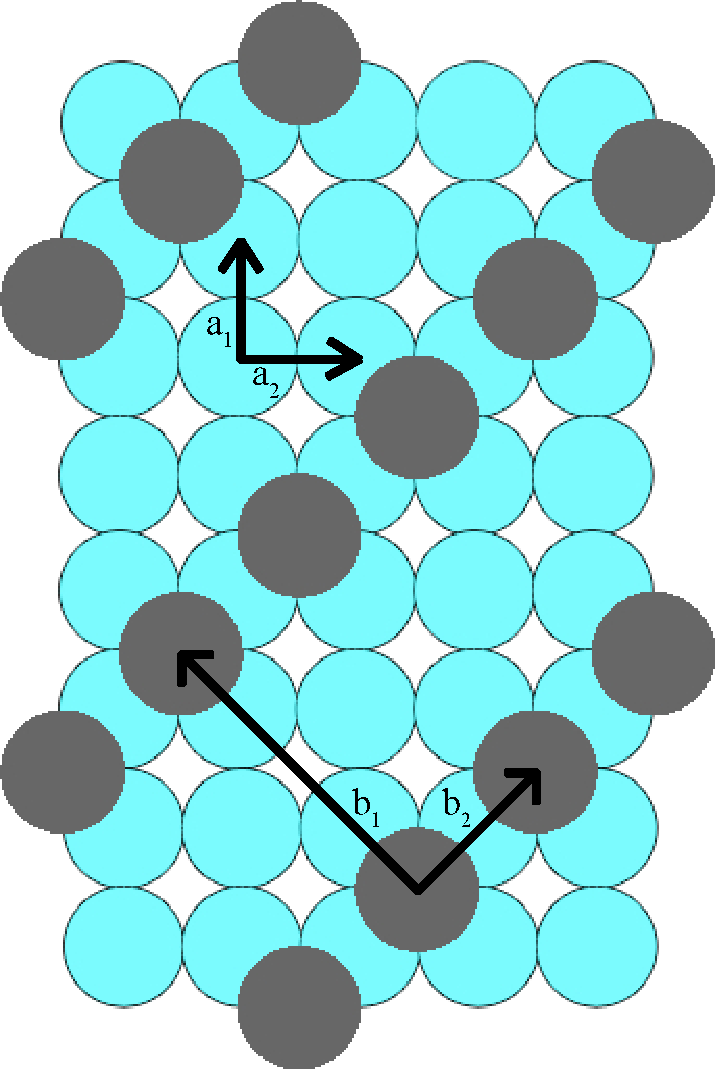
\includegraphics[width=0.2\linewidth]{img/superstructure.pdf}
       	&
       		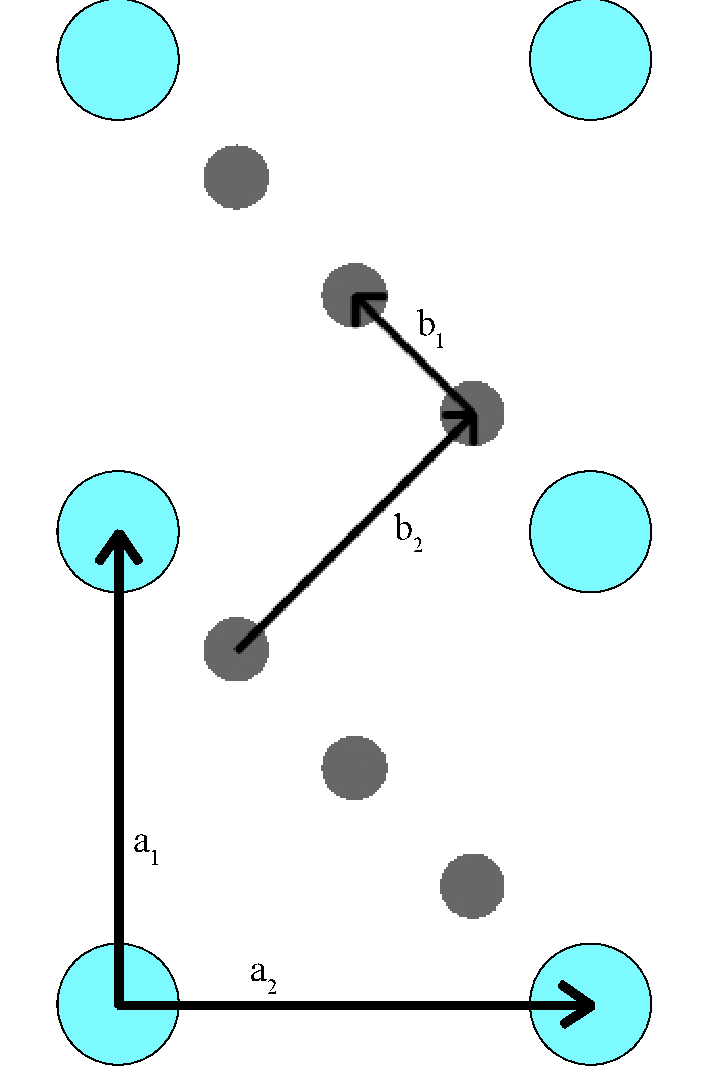
\includegraphics[width=0.2\linewidth]{img/superstructure2.pdf}
		  \end{tabular}
        \end{center}
        \caption{
			\small \textbf{(left)} A regular square lattice (e.g. Cu atoms) with lattice vectors $a_{1,2}$ and a  $(\sqrt{2} \times 2\sqrt{2})R45^\circ$ superstructure with vectors $b_{1,2}$.
			\textbf{(right)} The same lattice in the reciprocal space.
        }
        \label{fig:superstructure}
\end{figure}


\subsection{Kinematic Approximation}


 \bibliographystyle{unsrt}
\bibliography{FPbib}

\end{document}
